Primeiramente começamos com a apresentação da solução proposta (tarefa que está com o Jair), sem apresentar nenhum detalhe técnico nem nada parecido, apenas explicando o funcionamento da solução. 

Esta solução está organizada segundo a EAP (Estrutura analítica do projeto) apresentada na figura x, destacando os entregáveis e seus sub-sistemas ao longo de todo o projeto.

FIGURA DA EAP AQUI!

\section{Requisitos do sistema} % (fold)
\label{sub:requisitos_do_sistema}

% section requisitos_do_sistema (end)
\section{Alimentação} % (fold)
\label{sub:alimentação}
	Definição detalhada da solução em relação a alimentação (Luan)
% section alimentação (end)

\section{Navegação} % (fold)
\label{sub:automação}
	A solução referente à navegação possui enfoque principal no algoritmo de controle que trabalhará a trajetória a ser percorrida, a identificação de obstáculos e replanejamento da trajetória e a lógica de controle para retorno à base. Diversas possibilidades foram estudadas e analisadas, desde o planejamento de rota partindo com formato espiral, até trajetórias aleatórias com simples desvios de obstáculos.

	A partir e comparações e estudo de concorrentes, como o robô \textit{Roomba}\footnote{https://www.irobot.com.br/}, por exemplo, observou-se que na grande maioria, o sistema de navegação escolhido pelos fabricantes é baseado em trajetórias aleatórias. Segundo \cite{robo_limpeza_domesti}, a utilização de navegação aleatória garante um bom desempenho, já que com o passar do tempo, o robô consegue acessar o cômodo como um todo. Dessa forma, optou-se pela utilização de um algoritmo de navegação baseado em trajetória aleatória para o desenvolvimento do sistema \textit{R2-PI2}.

	Um dos grandes problemas encontrados na navegação é referente a volta à base por parte do robô. Identificar onde a base se encontra e traçar uma rota até a mesma é uma tarefa que necessita de algumas ferramentas, como a utilização de sinais e sensores para comunicação entre a base e o robô. Para isso, optou-se pela utilização de 3 (três) sensores infra-vermelho emitidos pela base com uma angulação de 45º entre eles, fazendo com que o robô possa identificar o sinal e navegar até sua fonte, a base.
% section automação (end)

\section{Estrutura e Locomoção do robô} % (fold)
\label{sub:alimentação}
	
	O robô, de forma autônoma, deve percorrer todo o cômodo escolhido para limpá-lo para isso deve ser desenvolvido todo o sistema de locomoção dele, incluindo as rodas, motor, caixa de redução e todo o estudo dinâmico relacionado. Foram cogitadas duas soluções para a estrutura do robô e sua forma de locomoção, de forma que a segunda solução foi escolhida. A escolha da segunda solução se justifica com base nos requisitos do sistema de sensoriamento quanto a posição de sensores pela estrutura e devido ao maior erro propagado pela primeira solução na navegação inercial do sistema. 

	\subsection{Solução 1} % (fold)
	\label{sub:solução_1}

		O robô seria composto de uma chapa retangular de alumínio de 400mm x 300mm x 5mm, que servirá como base para a distribuição e união dos componentes do projeto. Essa base retangular poderá ser usinada para outra forma caso haja necessidade de diminuição do tamanho do robô. O material escolhido para a base foi o alumínio pela sua leveza, resistência e preço. Sua área  de superfície é capaz de abrigar todos os componentes do aspirador e ainda possui espaços para criar novas soluções ou até mesmo de componentes para a refrigeração dos subsistemas do robô.

		O sistema de tração dessa base será feito por uma esteira tipo lagarta, muito utilizada em tanques de guerra. Esse sistema é bastante robusto e aguentaria o peso de todo a estrutura sem problemas. Isso tiraria a necessidade de colocar um sistema de suspensão.

		A estrutura do aspirador e seus componentes:

		\begin{itemize}
			\item 2 motores com caixa de redução ligados a chapa de alumínio;
			\item Os eixos que ligaram as rodas a chapa de alumínio serão feitos com aço e serão usinados nas pontas para fazer roscas que irão fixar as rodas;
			\item 4 engrenagens grandes que serão utilizadas como rodas;
			\item 2 engrenagens menores que irão ser ligadas direto nos dois motores;
			\item Conectores múltiplos, do tipo que se usa em chuveiros para ligar os eixos na chapa de alumínio;
			\item Correntes de bicicleta que ligaram as engrenagens e farão o papel de esteira.
		\end{itemize}

		Entre esses dois sistemas foi escolhido o segundo pela sua construção ser mais robusta e suporta mais os esforços que será submetido o robô. Um grande problema do primeiro sistema é que a sustentação da estrutura se daria no próprio eixo do motor, que é de plastico, o que poderia causar a quebra do sistema, já no segundo sistema a sustentação é feita nos eixos, que são feitos de aço.
		
		\begin{figure}[H]
			\centering
			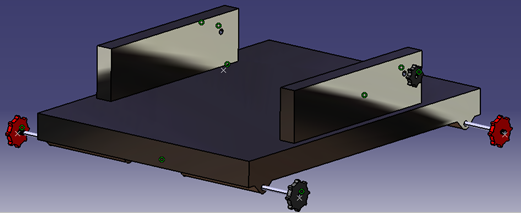
\includegraphics[scale=0.8]{figuras/rascunho_estrutura.png}
			\caption{Rascunho da estrutura - Solução 1}
			\label{img:rascunho1}
		\end{figure}

		\subsubsection{Orçamento da solução 1}

			As aquisições necessárias estão listadas abaixo:
			\begin{itemize}
				\item 2 motores com caixa de redução = R\$ 74 ,00
				\item 2 roldanas pequenas= R\$5,00
				\item 4 roldanas grandes = R\$ 16,00
				\item Corrente de bicicleta = R\$10,00
				\item Parafusos = R\$20,00
				\item Multi fixadores = R\$ 5,00
			\end{itemize}

		\subsection{Solução 2} % (fold)
		\label{sub:solução_2}
			
			O robô aspirador terá forma circular. Esse formato foi escolhido para facilitar as manobras de curvas, aumentando a área que ele irá percorrer. Outra vantagem que esse formato fornece é a questão do controle autônomo dele, assim facilita a distribuição dos sensores e o próprio controle do movimento do robô, pois resulta em menos erros. A estrutura do robô deve ser tal para suportar as cargas dos equipamentos do interior do robô como os sensores, motores, coolers e o sistema de sucção sem que sofra deformações. Além dessas forças deve-se também ser resistente à fadiga, já que estará sujeito a cargas contínuas e repetidas, e a impactos contra objetos ou paredes. Um material que já é utilizado em muitas aplicações pois apresenta boa propriedades é o Alumínio. A tabela a seguir mostra alguns valores das propriedades mecânicas do alumínio.

			\begin{figure}[H]
				\centering
				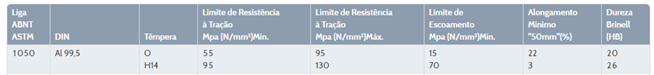
\includegraphics[scale=0.8]{figuras/tabela_estru1.png}
				\caption{Propriedades mecânicas do alumínio.}
				\label{img:rascunho1}
			\end{figure}

			Então será construída uma base circular de alumínio de 40 cm de diâmetro.

        	Com relação a movimentação do robô 3 rodas serão suficientes para garantir o equilíbrio. Duas rodas serão tracionadas uma livre.  A roda livre é do tipo esfera e as outras duas serão de um kit motor redução, que junto à roda está montado o motor com uma caixa de redução para aumentar o torque. A mudança de direção e giro do robô é realizada alternando a potência fornecida em cada roda ou invertendo o sentido de rotação, por exemplo para fazer com que ele gire para a esquerda, deve diminuir a potência da roda esquerda e manter a potência da roda direita. As figuras seguintes ilustram as rodas e motores utilizados.

        	\begin{figure}[H]
				\centering
				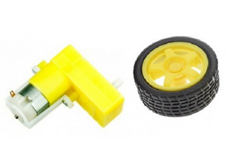
\includegraphics[scale=0.7]{figuras/motor_roda.png}
				\caption{Kit motor redução. Disponível em http://www.huinfinito.com.br/motores/787-motor-com-engrenagem-de-reducao-3-6v-90-graus.html?search\_query=roda\&results=7}
				\label{img:kit_motor}
			\end{figure}

			\begin{figure}[H]
				\centering
				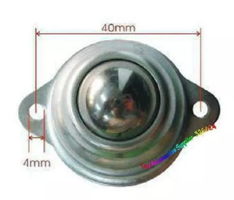
\includegraphics[scale=0.7]{figuras/esfera.png}
				\caption{Roda do tipo esfera. Disponível em http://produto.mercadolivre.com.br/MLB-772876471-roda-boba-robot-caster-esfera-roda-rodinha-pra-robotica-robo-\_JM}
				\label{img:esfera}
			\end{figure}

			As especificações da roda e do motor são mostradas na tabela \ref{tab:motor_red}:

			\begin{table}[H]
				\centering
				\caption{Especificação motor de redução}
				\label{tab:motor_red}
				\begin{tabular}{|c|c|}
					\hline
					\multicolumn{2}{|c|}{\cellcolor[HTML]{C0C0C0}\textbf{Especificação Motor}} \\ \hline
					\textit{\textbf{Tamanho}}                            & 69x37x22,7mm        \\ \hline
					\textit{\textbf{Peso}}                               & 29g                 \\ \hline
					\textit{\textbf{Formato}}                            & 90 graus            \\ \hline
					\textit{\textbf{Tensão de operação}}                 & 3 a 6V              \\ \hline
					\textit{\textbf{Relação de transmissão}}             & 1:120               \\ \hline
					\textit{\textbf{Velocidade a 3V(sem carga)}}         & 100 rpm             \\ \hline
					\textit{\textbf{Corrente a 3V(sem carga)}}           & 60 mA               \\ \hline
					\textit{\textbf{Corrente a 3V(com carga)}}           & 260 mA              \\ \hline
					\textit{\textbf{Torque a 3V}}                        & 1.20 kgf-cm         \\ \hline
					\textit{\textbf{Velocidade a 6V(sem carga)}}         & 200 rpm             \\ \hline
					\textit{\textbf{Corrente a 6V(sem carga)}}           & 71 mA               \\ \hline
					\textit{\textbf{Corrente a 6V(com carga)}}           & 470 mA              \\ \hline
					\textit{\textbf{Torque a 6V}}                        & 1.92 kgf-cm         \\ \hline
					\textit{\textbf{Diâmetro externo do eixo}}           & 5,4 mm "I"          \\ \hline
				\end{tabular}
			\end{table}

			\begin{figure}[H]
				\centering
				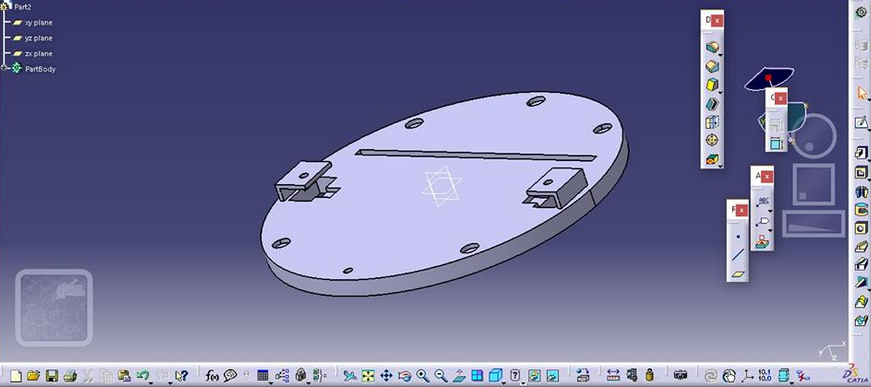
\includegraphics[scale=0.5]{figuras/estrutura_circular.png}
				\caption{Estrutura circular de integração dos subsistemas.}
				\label{img:estrutura_circular}
			\end{figure}

			\begin{table}[H]
				\centering
				\caption{Especificações roda tracionada}
				\label{tab:especificacoes_roda}
				\begin{tabular}{|c|c|}
					\hline
					\multicolumn{2}{|c|}{\cellcolor[HTML]{C0C0C0}\textbf{Especificação da Roda}}                 \\ \hline
					\textit{\textbf{Material}}                             & Roda plástica com pneu de borracha. \\ \hline
					\textit{\textbf{Diâmetro externo}}                     & 65 mm                               \\ \hline
					\textit{\textbf{Largura pneu}}                         & 26 mm                               \\ \hline
					\textit{\textbf{Diâmetro interno para engate do eixo}} & 5,4 mm "I"                          \\ \hline
				\end{tabular}
			\end{table}

			A parte superior da estrutura, ou seja, a tampa, será fabricada em PVC ou em acrílico. A escolha de um material plástico deve-se a facilidade de manuseio, facilitando molda-lo à forma desejada. Deixa a estrutura mais leve, fazendo com que o motor realize menos trabalho, e pode suportar valores altos de cargas, resistindo a impactos. O material acrílico (METACRILATO DE METILA) possui (densidade relativa de 1.19 g/cm3), resistente a água e boa resistência segundo a Figura \ref{img:acrilico}:

			\begin{figure}[H]
				\centering
				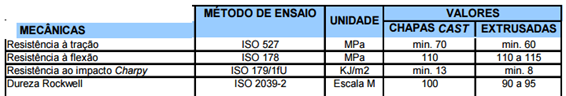
\includegraphics[scale=0.8]{figuras/tabela_acrilico.png}
				\caption{Valores de propriedades mecânicas do Acrílico. Adaptado de http://www.indac.org.br/arquivos/acrilico\_indac.pdf}
				\label{img:acrilico}
			\end{figure}

			Na tabela \ref{tab:pvc} são apresentados os valores referentes ao PVC.

			\begin{table}[H]
				\centering
				\caption{Valores das propriedades mecânicas do PVC}
				\label{tab:pvc}
				\begin{tabular}{|c|c|c|c|}
					\hline
					\textit{\textbf{Materiais}} & \textit{\textbf{\begin{tabular}[c]{@{}c@{}}Resistência a tração\\ (N/mm\textsuperscript{2})\end{tabular}}} & \textit{\textbf{\begin{tabular}[c]{@{}c@{}}Módulo de elasticidade\\ (kN/mm\textsuperscript{2})\end{tabular}}} & \textit{\textbf{\begin{tabular}[c]{@{}c@{}}Densidade\\ (kg/m\textsuperscript{3})\end{tabular}}} \\ \hline
					PVC                         & 55                                                                                       & 3.5                                                                                         & 1400                                                                          \\ \hline
				\end{tabular}
			\end{table}

			Ambos os materiais apresentam boa resistência à tração e podem ser aplicados ao projeto e irão proteger os circuitos, baterias, motores e outros equipamentos sensíveis em seu interior. A placa de acrílico ou de PVC cortado e usinado para se encaixar na estrutura montada utilizando parafusos e porcas. Os parafusos irão facilitar o trabalho de encaixe e desencaixe da tampa de acrílico para ajustes e limpezas das peças, além de fixar melhor. Se a tampa fosse colada na estrutura não haveria essa possibilidade.

			\subsubsection{Orçamento}

			\begin{itemize}
				\item 2 Kit motor redução – R\$ 49,80
				\item 1 roda esférica – R\$ 17,95
				\item Chapa de alumínio – R\$ 24,90 
				\item Chapa de PVC – 220cm x 110cm x 10mm - R\$ 17,00
				\item Chapa de acrílico 100cm x 50cm x 2mm – R\$ 54,90
			\end{itemize}
		% subsection solução_2 (end)

	% subsection solução_1 (end)
% section alimentação (end)

\section{Estrutura da Base} % (fold)
\label{sec:estrutura_da_base}
	
	O robô terá uma base de recarga automática responsável pelo guiamento do sistema pelo ambiente, pelo recarregamento da bateria e por abrigar e alimentar o Raspberry Pi que fará os cálculos de movimento do sistema.

	\subsection{Solução} % (fold)
	\label{sub:solução}
		
		O requisito é que o robô ao identificar que está com bateria baixa irá seguir para a base seguindo o sinal emitido por ela. A estrutura da base não necessita ter grande porte, por ser fixa e possuir menos equipamentos em seu interior. A base terá uma carcaça quadrada de dimensões 250x250x200mm, como se fosse uma caixa e assim como o robô aspirador, será feito em acrílico ou PVC pela leveza, resistência e custo. Como é uma peça de plástico também evitará condução de corrente, mantendo a proteção do usuário contra choques.  O conector será do tipo magnético, pois no momento em que for ocorrer o encaixe entre as peças do conector, esta possa ser feita de modo mais certeiro e ficará na face oposta à que fica apoiada na parede.

		\begin{figure}[H]
			\centering
			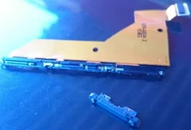
\includegraphics[scale=0.8]{figuras/conector_mag.png}
			\caption{Conectores magnético modelo Sony Xperia.}
			\label{img:conectores}
		\end{figure}

		\begin{figure}[H]
			\centering
			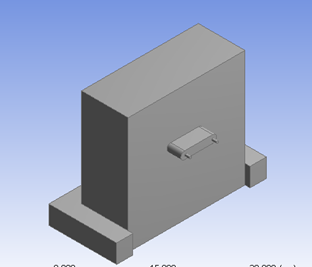
\includegraphics[scale=0.8]{figuras/estrutura_base.png}
			\caption{Estrutura da base de recarga.}
			\label{img:estrutura_base}
		\end{figure}	

	\subsection{Orçamento} % (fold)
	\label{sub:orçamento}
		
		\begin{itemize}
			\item Chapa de alumínio – R\$ 24,90 
			\item Chapa de PVC – 220cm x 110cm x 10mm - R\$ 17,00
			\item Chapa de acrílico 100cm x 50cm x 2mm – R\$ 54,90
			\item Conectores de carga Xperia Z3 – R\$ 55,00
		\end{itemize}	
	% subsection orçamento (end)	

	% subsection solução (end)
% section estrutura_da_base (end)

\section{Sucção} % (fold)
\label{sub:aspirador}
	
	Dentro dos principais objetivos, é necessário construir de forma objetiva um aspirador de pó. Deve-se projetar um sistema de sucção eficiente para que sugue desde de partículas de poeiras a resto de alimentos, estudo da dinâmica do processo, ou seja, o fluxo de ar dentro do motor do aspirador. Há dois tipos principais de modelos para ser utilizado em aspiradores de pó, um é o mais clássico utilizando ventiladores controlados por motores elétricos fazendo com que a pressão no interior do motor seja menor que a do ambiente e a diferença de pressão força o ar a entrar no aspirador seguindo até encontrar uma saída. Um filtro é colocado antes do ventilador para que seja separado a poeira do ar. O outro tipo é chamado de ciclone e não necessita de um filtro, pois pelo mesmo princípio da diferença de pressão o ar é sugado mas segue em uma trajetória helicoidal em torno de um cone e por efeito de força centrípeta a poeira é jogada para as paredes do aspirador e depois se depositam do inferior do aspirador onde são removidas, enquanto o ar percorre na direção contrária.

	\subsection{Solução} % (fold)
	\label{sub:solução}
		
		Para o projeto foi escolhido o primeiro modelo do ventilador com filtro, pois  é uma solução com um custo menor e de fácil implementação se comparado ao sistema ciclone. Serão integradas nesse sistema escovas abaixo da linha de sucção, conhecidas como vassouras mágicas, que irão facilitar o transporte e direcionar a poeira para dentro do aspirador. Serão escolhidos dois coolers comerciais com uma vazão de ar por volta de 160 m\textsuperscript{3}/h, que serão colocados lado a lado dentro de um sistema hermeticamente fechado.

		A geometria do sistema busca diminuir a área de escoamento para aumentar a velocidade do fluído na ponta de sucção, utilizando do principio de conservação do fluxo de massa do sistema. O sistema de vedação será construído utilizando acrílico colado e mangueiras sanfonadas. Também será utilizado um motor para o acionamento da escova. Para o armazenamento do pó, será projetada uma caixa retangular de plástico com tampa. No momento da limpeza do depositório, o proprietário do aspirado deve apenas desencaixar a parte móvel, retirar as impurezas e encaixar novamente na tampa.

		O dispositivo de sucção da poeira está baseado na predição fornecida pela Equação da Continuidade. A equação descreve que o fluxo de massa que entra no sistema e o que sai no sistema é igual, de forma que a diminuição da seção transversal da tubulação causa um aumento da velocidade do escoamento, que por usa vez vai ter uma capacidade maior de arrastar partículas para dentro do sistema. Por sua vez, uma velocidade maior em um escoamento causa uma diminuição da pressão pelo princípio de Bernoulli e essa variação da pressão causa uma força que auxilia a aspiração de partículas.

		Os dados relativos ao fluxo de massa e potência dos coolers comerciais é muito limitado. Assim o dimensionamento do sistema será realizado utilizando uma simulação de base no Ansys em conjunto com experimentos empíricos em protótipos simplificados. Para primeira análise, foi realizada uma simulação com as condições de contorno definidas pelo fluxo de massa constante na entrada e na saída, com um valor de 0,026Kg/s ou  cerca de 50 CFM. A simulação mostrou uma velocidade de saída do escoamento de 5 m/s e a velocidade de entrada do ar de 19 m/s.

		\begin{figure}[H]
			\centering
			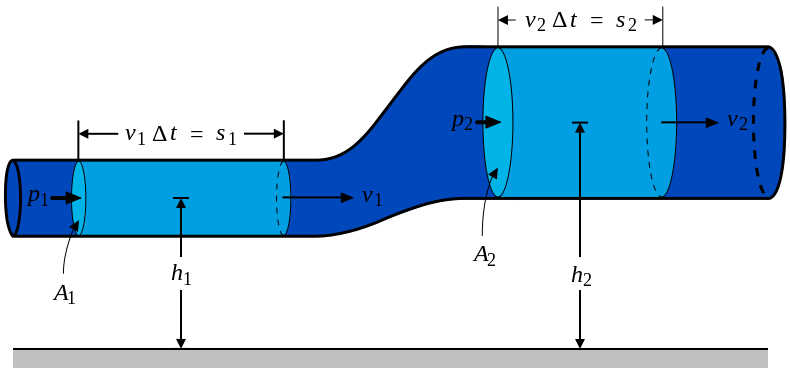
\includegraphics[scale=0.4]{figuras/succao.png}
			\caption{Demonstração da equação da continuidade, equação que descreve a conservação de massa do escoamento.}
			\label{img:succao}
		\end{figure}

		$\frac{v^{2}}{2} + gh + \frac{p}{\rho} = constante$ ou $\frac{\rho v^{2}}{2} + \rho gh + p = constante$

		$v$ = velocidade do fluido ao longo do condutor

		$g$ = aceleração da gravidade
		
		$h$ = altura em relação a um referencial
		
		$p$ = pressão ao longo do recipiente
		
		$\rho$ = massa específica do fluido

		Segue a equação da continuidade na sua forma de integral:

		$\frac{dq}{dt} + \iint_{s}^{ }j . dS= \sum$, onde

		$S$ é qualquer superficie fechada imaginária, com um volume V

		$\iint_{s}^{ }dS$ se refere a integral de superficie sobre a superficie fechada

		$q$ é o amontoado total do volume

		$j$ é o fluxo de q

		$t$ é o tempo


		A analise do fluxo de massa realizada no software \textit{Ansys} está apresentada na Figura \ref{img:analise_fluxo}.

		\begin{figure}[H]
			\centering
			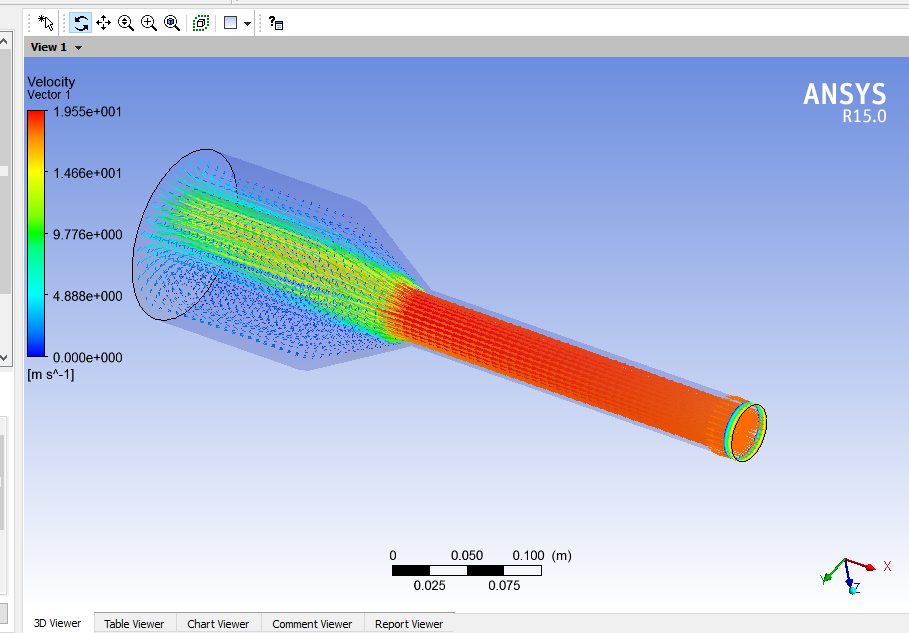
\includegraphics[scale=0.4]{figuras/analise_fluxo.png}
			\caption{Simulação do Ansys com o fluxo de massa de um cooler comercial.}
			\label{img:analise_fluxo}
		\end{figure}

		\subsection{Orçamento} % (fold)
		\label{sub:orçamento}
			
			A lista de peças necessárias para o sistema de sucção é:
			\begin{itemize}
				\item Dois coolers de 120mm x 120mm - R\$ 20,00
				\item Chapa de Poliestireno Cristal (Parece Acrílico) 100cm x 50 cm x 2 mm - R\$ 40,00
				\item Cola para Acrílico Reverstsul 100ml - R\$ 26,00
				\item Mangueira de saída de Ar (secadoras) - R\$ 52,00
				\item Vasilha de plastico - R\$ 10,00
				\item 4 Aneis de vedação - 4 x R\$ 8,00
				\item Espuma para filtro de poeira - R\$ 10,00
			\end{itemize}
		% subsection orçamento (end)


	% subsection solução (end)
% section aspirador (end)

\section{Instrumentação} % (fold)
\label{sub:instrumentação}
	Definição detalhada da solução em relação a instrumentação. (Kaio)
% section instrumentação (end)

\section{Comunicação} % (fold)
\label{sub:comunicação}
	De acordo com o apresentado nesta documentação de projeto, a solução proposta envolve diversos módulos funcionais, como o robô em si, a base fixa, e o sistema de controle. A partir de uma visão de alto nível do projeto, como a apresentada na Figura \ref{img:arq_comu}, é possível observar de maneira clara os módulos que deverão se comunicar para garantir o funcionamento do sistema como um todo.

	\begin{figure}[H]
		\centering
		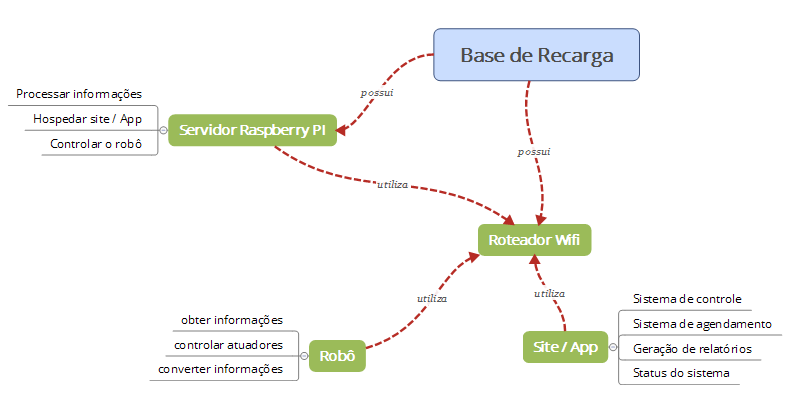
\includegraphics[scale=0.8]{figuras/arquitetura_comunicacao.png}
		\caption{Arquitetura de comunicação do sistema}
		\label{img:arq_comu}
	\end{figure}

	Com o objetivo de garantir que a solução seja confiável e resistente a situações críticas, como a falta de internet, por exemplo, o sistema foi planejado para disponibilizar uma sub-rede interna, tendo como fonte a base de recarga do robô. Cada módulo que necessita de comunicação deverá se conectar a rede, viabilizando o funcionamento do sistema mesmo em momentos com falha de internet, já que todos os envolvidos compartilham o mesmo ambiente.

	A comunicação entre o robô (\textit{arduino}) e a base (raspberry) fará uso desta rede wifi, a partir da utilização de um módulo wifi, o \textit{arduino} poderá acessar a rede, possibilitando a comunicação via tcp/ip. Já a \textit{raspberry} se conectará a rede via cabo \textit{ethernet}.

	O roteador utilizado é da familia D-link, seguindo o protocolo de certificação WPA2, que utiliza o EAS (Advanced Encryption Standard), como sistema de encriptação. Segundo \cite{wpa2}, este protocolo possui uma confiabilidade bem maior que a encontrada em seu antecessor, WPA. Ainda de acordo com \cite{wpa2}, este sistema de segurança envolve um algoritmo de criptografia robusto, utilizando chaves de 128 a 256 bits maximizando a segurança da rede.


	O núcleo da rede, ou seja, o ponto central da comunicação do sistema se encontra na base de recarga do robô, que está detalhada no tópico a seguir.

	\subsection{Base de regarga}

	A base de recarga do robô sustentará todo o sistema de inteligência da solução, assim como a sub-rede que possibilitará a comunicação entre os módulos. Será utilizada uma \textit{raspberry PI} como servidor central do sistema, processando e controlando toda a solução. O servidor será implementado utilizando a tecnologia Ruby on Rails, no sistema operacional \textit{Raspbian} (Debian).

	Além da sustentação da \textit{raspberry}, é necessário sustentar um roteador D-link 524 para implementação e sustentação da rede wifi que será utilizada como meio de comunicação do sistema, e 3 (três) emissores infra-vermelho, utilizados para retorno do robô à base.
	
% section comunicação (end)

\section{Interface} % (fold)
\label{sub:interface}
	Definição detalhada da solução em relação a interface. (Ricardo)
% section interface (end)
